\documentclass[10 pt, A4paper]{article}
\title{Informe para el Trabajo Práctico Especial - Programación III}
\author{Cagliolo, Camilo \& Fonzo Baniles, Luca}
\date{02/07/2023}
\usepackage[utf8]{inputenc}
\usepackage[skip=5pt, indent = 10pt]{parskip}
\usepackage[hoffset=0pt,voffset=0pt,]{geometry}
\usepackage{fancyhdr}
\usepackage{csquotes}
\usepackage{graphicx}
\usepackage{amsmath,amssymb}
\usepackage{hyperref}
\usepackage[spanish]{babel}


\usepackage{multirow}
\setlength{\arrayrulewidth}{0.5mm}
\renewcommand{\arraystretch}{2}

\usepackage{listings}
\usepackage{color}

\definecolor{dkgreen}{rgb}{0,0.6,0}
\definecolor{gray}{rgb}{0.5,0.5,0.5}
\definecolor{mauve}{rgb}{0.58,0,0.82}

\lstset{frame=tb,
	language=Java,
	aboveskip=3mm,
	belowskip=3mm,
	showstringspaces=false,
	columns=flexible,
	basicstyle={\small\ttfamily},
	numbers=none,
	numberstyle=\tiny\color{gray},
	keywordstyle=\color{blue},
	commentstyle=\color{dkgreen},
	stringstyle=\color{mauve},
	breaklines=true,
	breakatwhitespace=true,
	tabsize=3
}

\begin{document}
	\pagestyle{fancy}
	\fancyhead{}
	\fancyhead[RO]{\textbf{TPE - Programación III}}
	\fancyhead[RE,LO]{\thepage}
	\fancyfoot{}
	
	\maketitle
	\section*{Consigna}
	\begin{displayquote}
		\textit{Las autoridades de una ciudad deciden construir una red de subterráneos para resolver los constantes problemas de tráfico. La ciudad ya cuenta con N estaciones construidas, pero todavía no tienen ningún túnel que conecte ningún par de estaciones entre sí. La red de subterráneos que se construya debe incluir a todas las estaciones (es decir, que de cualquier estación H pueda llegar a cualquier otra estación J, ya sea de manera directa o atravesando otras estaciones). Sin embargo, debido al acotado presupuesto, las autoridades desean construir la menor cantidad de metros de túnel posibles . Para esto han calculado cuantos metros de túnel serían necesarios para conectar de manera directa cada par de estaciones existentes.}
	\end{displayquote}
	\subsubsection*{Objetivo}
	El objetivo es resolver el problema planteado mediante dos técnicas algorítmicas distintas: Backtracking y Greedy. Luego se deberán comparar los resultados teniendo en cuenta distintas métricas que permitan visualizar, mínimamente, la calidad de la solución y el costo de obtener dicha solución, con ambas técnicas.
	\section*{Solución}
	
	Los objetos a ser representados -estaciones y túneles- en el sistema se adaptan perfectamente a una estructura de datos de tipo grafo. Para ello se utilizará el 
	
	\subsection*{Algoritmo greedy}
	
	\textbf{Estrategia.} La estrategia empleada para la implementación del algoritmo greedy consistió en seleccionar para cada vértice del grafo el arco más corto disponible; los arcos disponibles son aquellos arcos que no tuvieran como vértice destino un vértice con un arco ya asignado.
	
	\textbf{Complejidad temporal.} Como consecuencia del funcionamiento del algoritmo, la estrategia greedy hace un repaso por cada vértice y a su vez, por cada vértice, el proceso de selección repasa todos los otros vértices que aún no han sido visitados, generando así una complejidad temporal de $O(n^2)$, de tipo polinomial, siendo $n$ la cantidad de vértices en el grafo.
	
	\subsection*{Algoritmo de backtracking}

	\textbf{Estrategia.} La estrategia consistió en construir una solución seleccionando un túnel por cada estación de forma sucesiva hasta quedarse sin estaciones que conectar. Dentro de cada paso, el algoritmo explora dos opciones: por un lado, si es posible, elige volver a la estación anterior sin construir ningún túnel. Por el otro, explora la construcción de un túnel nuevo hacia una estación que esté aún sin visitar (esto evita los ciclos en el grafo, que implicarían la construcción de túneles de más que no aportarían una nueva conexión). Esta exploración se realiza tomando como estación inicial a cada una de las estaciones, y puede visualizarse en la Figura \ref{tree}.
	
	\begin{figure}[h]
		\centering
		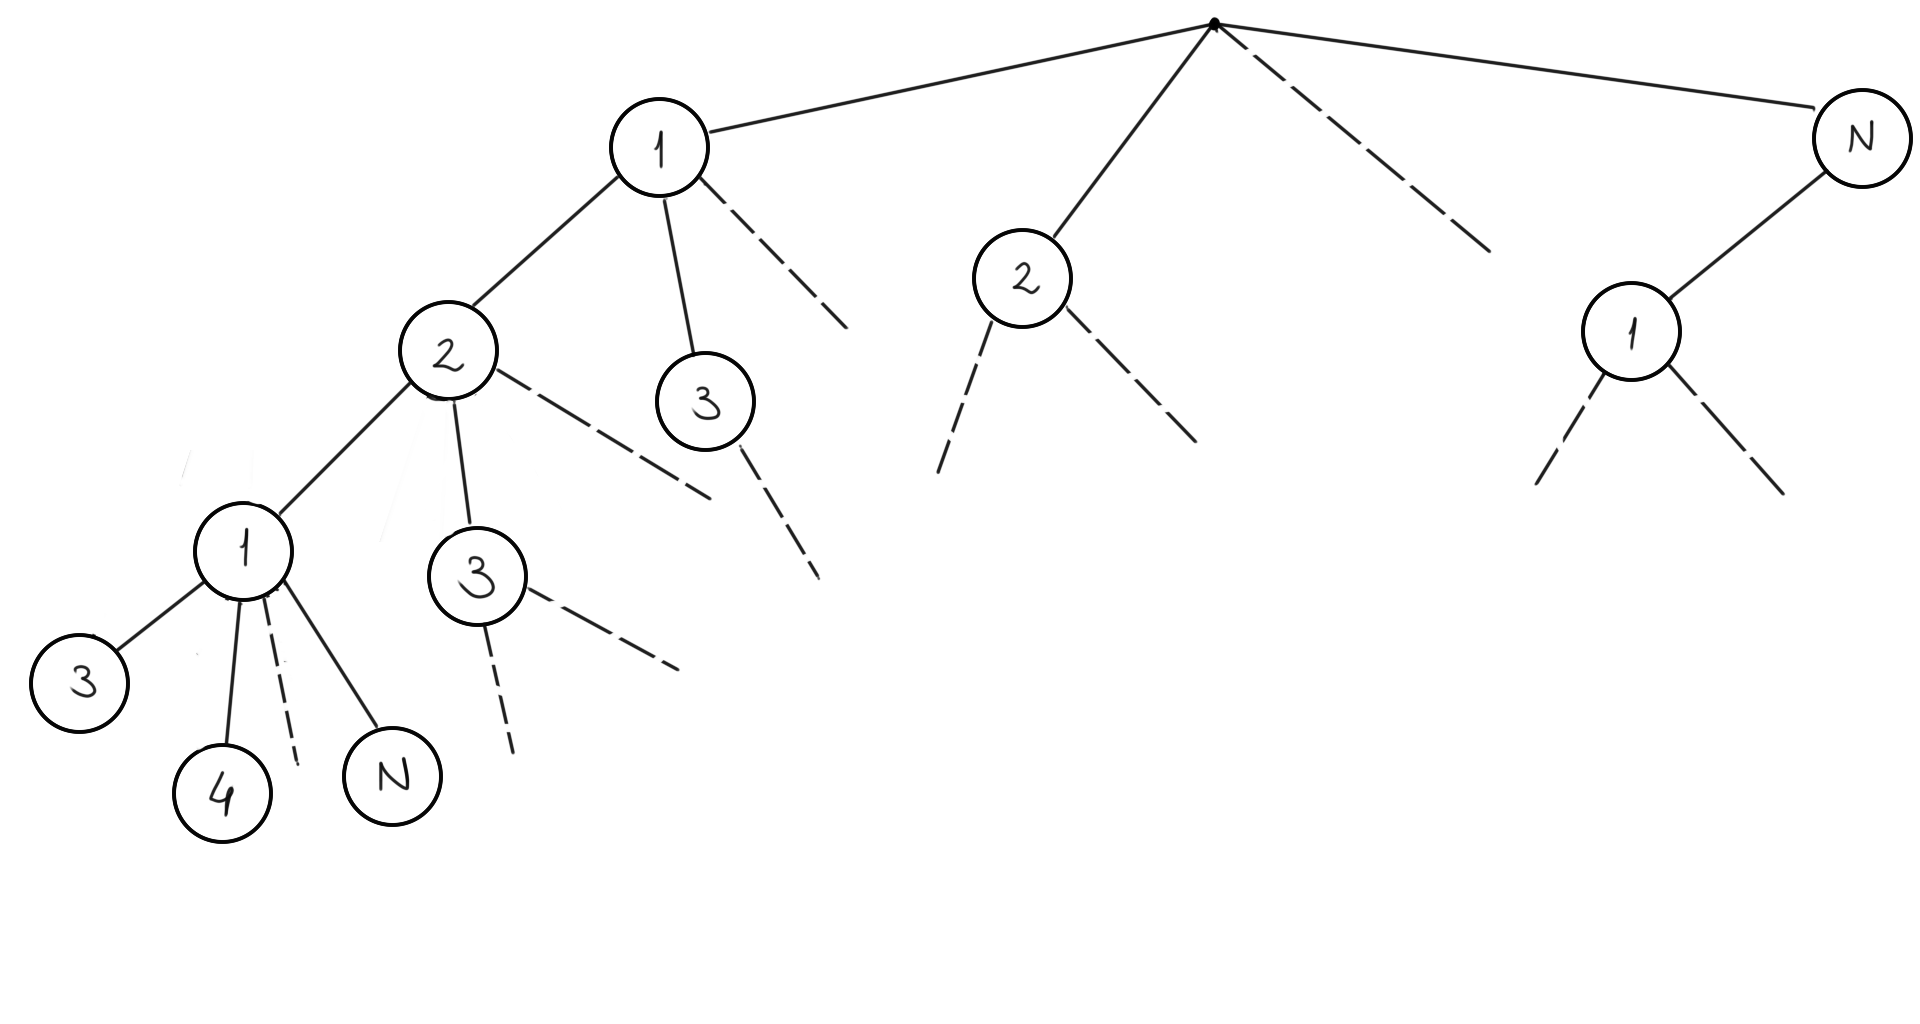
\includegraphics[scale = 0.18]{Árbol de exploración.png}
		\caption{Árbol de exploración para el algoritmo de backtracking.}
		\label{tree}
	\end{figure}
	
	\textbf{Complejidad temporal.} El carácter recursivo de la implementación con la estrategia de backtracking asegura la construcción de todas las combinaciones posibles de $n-1$ túneles para $n$ estaciones, visitando una por vez. La solución consiste en una lista de $n-1$ túneles, por lo que la cantidad de combinaciones posibles es $(n-1)!$. Como la exploración se ejecuta tomando como punto inicial a cada una de las estaciones, esto se repite $n$ veces, dando un total de $n!$ ciclos sin poda. En otras palabras, la implementación tiene una complejidad computacional $O(n!)$.
	
	Como el problema se trata de minimizar la distancia total, la condición fundamental de poda es asegurar que la construcción actual sea más corta que la última solución encontrada, pues de lo contrario no tiene sentido seguir construyendo: las distancias son cantidades siempre positivas. Esto permite acortar el tiempo de ejecución eliminando varias exploraciones subóptimas.
	
	\section*{Análisis}
	El cuadro \ref{table} muestra una tabla comparativa con las diferencias entre los algoritmos con estrategias \textit{greedy} y \textit{backtracking}, analizando el tiempo de ejecución y la cantidad de ciclos, además de la complejidad computacional teórica.
	
	\begin{table}[h!]
		\centering
		\begin{tabular}{|p{3.8cm} | p{3.5cm} | p{3.6cm} | p{3.6cm}|}
			\hline
			Algoritmo & Dataset 1 & Dataset 2 & Dataset 3 \\
			\hline
			\multirow{3}{1em}{Greedy $O(n^2)$} & Tiempo: $0.248\,ms$ & Tiempo: $0.499\,ms$& Tiempo: $0.466\,ms$ \\ & Ciclos: $14$ & Ciclos: $27$ & Ciclos: $104$ \\ & Distancia total: $80\,km$ & Distancia total: $145\,km$& Distancia total: $520\,km$ \\
			\hline
			\multirow{3}{1em}{Backtracking $O(n!)$} & Tiempo: $1.609\,ms$& Tiempo: $15.83\,ms$& Tiempo: $10.45\,min$\\ & Ciclos: $89$ & Ciclos: $1955$ & Ciclos: $1.182.011.744$ \\ & Distancia total: $55\,km$& Distancia total: $135\,km$& Distancia total: $450\,km$\\
			\hline
		\end{tabular}
		\caption{Comparación de costos y calidad de solución entre las dos estrategias.}
		\label{table}
	\end{table}
	
	\section*{Conclusiones}
	A partir de lo analizado y lo trabajado en clase, es posible llegar a las siguientes conclusiones:
	\begin{itemize}
		\item[$\circ$] Los algoritmos de tipo greedy pueden otorgar soluciones que están muy cerca de ser la óptima, consumiendo muchos menos recursos que su contraparte de backtracking. Sin embargo, no hay forma de saber a priori qué tan óptima es la solución, pues eso dependerá íntegramente del problema particular.
		\item[$\circ$] Los algoritmos de backtracking aseguran la solución más óptima, por lo que si el costo computacional es pagable, podría ser preferible.
		\item[$\circ$] Una combinación de ambas metodologías podría permitir podar gran parte del árbol de búsqueda del algoritmo de backtracking, utilizando como filtro los resultados del algoritmo greedy.
		\item[$\circ$] El tiempo de ejecución para los algoritmos de backtracking escala enormemente con el tamaño de la entrada, volviéndose rápidamente una estrategia inviable.
	\end{itemize}
	
	
\end{document}